%\begin{document}
\documentclass[a4paper,12pt]{article}
\usepackage{indentfirst}%paragrafo no primeiro tb
\usepackage[english,brazil]{babel}
\usepackage[utf8]{inputenc}
\usepackage{amsmath}
\usepackage{graphicx}
\usepackage{fancyhdr}
\usepackage{url}
\renewcommand{\baselinestretch}{1.5}
\usepackage{setspace}%%%% pacote para espaço duplo
\usepackage{titling}
\usepackage{geometry}
\usepackage{amsmath}
\usepackage{amssymb}
\usepackage{subfigure}
\usepackage{multirow}
\usepackage[table]{xcolor}
\usepackage{fullpage}
\usepackage[backend=bibtex,style=ieee,sorting=none]{biblatex}
\bibliography{refs}


\newcolumntype{C}{>{\centering\arraybackslash}p{1em}}

% FAPESP pede "tipo equivalente a Times New Roman"
% Acho que na verdade eles só estão preocupados com o tamanho da fonte
% A diferença entre a fonte padrão do LaTeX e times é pequena
%\usepackage{times}

\title{\textbf{Controle de Estabilização de Caminhada de Robô Humanoide
}\\
\vspace{30px}
\normalsize \textbf{Projeto de Pesquisa para Iniciação Científica}\\
 \textbf{Departamento de Engenharia Mecânica-Aeronáutica}\\
 \textbf{Instituto Tecnológico de Aeronáutica -- ITA}
 }






%%%%


\author{\textbf{Beneficiário:} Reynaldo Santos de Lima\\
\textbf{Orientador:} Marcos Ricardo Omena de Albuquerque Maximo\\
 } %\\

%%%%%%%

\date{\today}
% ADD THE FOLLOWING COUPLE LINES INTO YOUR PREAMBLE
\let\OLDthebibliography\thebibliography
\renewcommand\thebibliography[1]{
  \OLDthebibliography{#1}
  \setlength{\parskip}{0pt}
  \setlength{\itemsep}{0pt plus 0.3ex}
}


\begin{document}
\maketitle

%\newpage
%\maketitle

\selectlanguage{brazil}
\newpage
\doublespacing

%\thispagestyle{empty}
\begin{abstract}
Neste trabalho pretende-se desenvolver um pé robótico para com o objetivo de reduzir o gasto energético da marcha de  um robô humanoide de baixo custo (Robotis OP2). Esse trabalho será realizado no  Laboratório de Sistemas Computacionais Autônomos (LAB-SCA), onde  existe um estudo de caminhada do Robotis OP2 . Em uma primeira etapa, será realizada uma identificação de parâmetros pela técnica de cinemetria em conjunto com o Laboratório de Biomecânica, Robótica e Simulação Computacional (LBRSC)  para a validação de um simulador existente.
A questão energética será abordada de tal maneira que uma nova geometria e novos materiais sejam utilizados para o desenvolvimento de um novo pé para o robô em operação permitindo realizar um rolamento natural semelhante ao que acontece na marcha humana. Para isso, primeiro será desenvolvido um simulador do novo pé robótico  e depois um projeto mecânico do novo pé com forma otimizada, ou seja, um pé leve que mantenha sua rigidez e que permita o rolamento e amortecimento, diminuindo não só a energia gasta como também as forças de impacto.
Para análise desse novo comportamento serão determinadas as forças de impacto por sensores de pressão. Em seguida, a fim de validar esse novo pé robótico será proposto um algoritmo de caminhada que considere esse rolamento que será implementado no robô.
%%%
\end{abstract}
%%%
%\selectlanguage{brazil}
%%%%%
\newpage
%%%%%%
\section{Introdução, Justificativa e Síntese da Bibliografia Fundamental}
%\label{secao:enunciado_problema}



No contexto da robótica móvel existem diversos problemas a serem abordados e um que se destaca é o estudo de robôs humanoides, especificamente a questão da caminhada. Esse movimento é uma ação complexa do ponto de vista de controle, devido às não linearidades, a subatuação e  de ter alta dimensão dinâmica, ou seja, muitos graus de liberdade. Representando um grande desafio às técnicas de controle de última geração \cite{tedrake2005}.

Uma primeira questão a ser analisada é a estabilidade estática dos bípedes é assegurada pela projeção de centro de massa (CM) no solo dentro de um polígono de suporte, definido na Literatura como a envoltória convexa dos pontos de contato no solo. Consequentemente, na estática, as forças de reação do solo atuam na vertical no ponto que equivale à projeção do CM para equilibrar as forças e momentos gerados pela gravidade, sendo o centro de pressão (CP) o ponto resultante das forças de reação.

Para desenvolver uma caminhada estável e rápida em robôs bípedes é necessário considerar os efeitos dinâmicos sobre o CP. Um conceito popular nesse contexto  utilizado é o Zero Moment Point (ZMP), que pode ser encarado  como o ponto no solo onde as forças de reação devem atuar para estabilizar o mecanismo bípede \cite{vukobratovic2004} assim, quando o ZMP estiver dentro do polígono de suporte, este coincide com o CP.

Quando em regime dinâmico o CM e o CP não coincidem, mas a aceleração do corpo auxilia na obtenção do equilíbrio. Por isso, na prática, para preservar a estabilidade basta delinear o movimento de maneira que o ZMP esteja sempre dentro do polígono de suporte. Na marcha há sempre um pé em contato com o solo em algum momento da caminhada e isso auxilia na transição para o apoio seguinte.

Como robôs humanoides têm muitos graus de liberdade e sua dinâmica é não linear, o movimento se torna complexo por isso são usados modelos de ordem reduzida.  Por exemplo, com o 3D Linear Inverted Pendulum Model (3D-LIPM)\cite{kajita2001} pode se obter a trajetória do CM e depois, por cinemática inversa, determinar os ângulos das juntas durante a caminhada. Por causa das simplificações do modelo, frequentemente usam-se estratégias de realimentação e compensação de erro de dinâmica para o robô ter estabilidade \cite{yoshiike2009}.


O que torna o robô humanoide tão atrativo é o fato de haver semelhança física com o ser humano, facilitando a interação com ferramentas e ambientes desenvolvidos para o uso humano. Porém a caminhada e a corrida estão longe de ser semelhante ao do ser humano, tornando-se um dos assuntos atuais da robótica móvel principalmente do ponto de vista energético. Por exemplo,  um  robô humanoide  avançado Asimo \cite{yoshiike2009}, que  utiliza o método do LIMP, gasta 10 vezes mais energia do que o ser humano \cite{tedrake2005} para caminhar.  

Um dos fatores responsáveis dessa enorme diferença de gasto energético é o fato do pé humano rolar no chão durante  cada etapa de caminhada, mais ou menos análoga a uma roda, o CP avança no chão girando em torno de um ponto fixo. 

\textit{Adamczyk et al.} examinaram o gasto energético da caminhada para diferentes curvaturas do pé, construindo uma bota que restringe o movimento do tornozelo e varia o raio do arco rígido referente à sola \cite{adamczyk2006}. Por fim, mediu  o trabalho e o taxa metabólica para o redirecionamento do CM durante a marcha, em dez indivíduos caminhando com sete raios de diferentes curvaturas da bota.

Comparando com um modelo simples de caminhada dinâmica, inferiu que pés rolantes com curvatura de 30\% do comprimento da perna  são energeticamente vantajosos para caminhar. Apesar desse movimento de rolamento parecer ajudar na economia de energia durante a marcha, os mecanismos dele não são claros. 

Novamente \textit{Adamczyk et al.} desenvolvem um modelo de caminhada dinâmica que prevê os efeitos energéticos ao alterar o comprimento do pé e o raio do pé \cite{adamczyk2013}. Realizando experimentos em oito indivíduos com o dispositivo desenvolvido em \cite{adamczyk2006}. O modelo do rolamento sugeriu que o trabalho da transição dos passos é pouco sensível ao tamanho do raio do arco do pé e varia aproximadamente com o quadrado do comprimento do pé.

No Brasil há pesquisadores abordando o estudo de bípedes. \textit{Siqueira e Terra} para obterem uma marcha antropomórfica utilizam controle não linear  \cite{terra2006} . \textit{Bianchi et al.} propõem aprendizagem por reforço para encontrar uma maneira automática de ajustar os valores dos parâmetros para a marcha de um humanoide \cite{bianchi2017}. 

O grupo de pesquisa do Laboratório de Sistemas Computacionais Autônomos (LAB-SCA) do ITA tem desenvolvido estudos na área de caminhada de robôs humanoides\cite{max22,max25,max27,max28,tesemarcos}.
No trabalho mais recente \cite{tesemarcos}, investigaram-se formulações baseadas em  Controle Preditivo  que permitem ao robô decidir a trajetória do CM, as posições dos pés e durações dos passos.

 Essas formulações demonstraram expandir consideravelmente a margem de tolerância e perturbações do robô (i.e. o robô é capaz de tomar empurrões muito mais fortes sem cair) em comparação a uma formulação do estado da arte que trabalha com duração fixa de passo \cite{max30}. Essa característica foi comprovada tanto em simulações simplificadas usando o consagrado modelo de pêndulo invertido \cite{kajita2001} para modelar o robô, quanto no simulador de robótica Gazebo, onde foi utilizado um modelo de simulação realista do robô humanoide Robotis OP2, desenvolvido pelo grupo a partir de dados do fabricante e de resultados de ensaios com os atuadores \cite{max27}. 
 
Uma desvantagem da caminhada desenvolvida pelo LAB-SCA nos robôs humanoides Robotis OP2 e Chape (robô humanóide projetado pelo LAB-SCA) mostrados nas figuras 1(a) e 1(b), respectivamente, é o alto gasto energético. Devido aos pés serem chapas retangulares e sem nenhum mecanismo de amortecimento, gerando muita vibração estrutural. 

\begin{figure}[!htb]
\centering
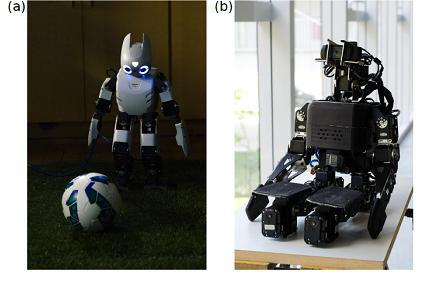
\includegraphics{img10}
\caption{Modelo de robôs humanóides do LAB-SCA, a) Robotis OP2 b) Chape.}
\label{Rotulo}
\end{figure}

Diferentes aspectos são abordados no atual estágio de desenvolvimento de pés robóticos, desde a forma geométrica dos pés à utilização de materiais flexíveis que possuem alto grau de amortecimento já que durante a caminhada bípede  deve-se levar em consideração a mudança de suportes (apoios), o que ocasiona muitas colisões fazendo a estrutura vibrar durante a caminhada.

O robô bípede JOHNNIE \cite{jonhie2006} tem os pés equipados com um mecanismo de amortecimento de impacto. Este mecanismo consiste de um elemento de contato em cada canto do pé. Sendo que este elemento tem uma alta deformação na direção vertical e uma camada de borracha com alto coeficiente de atrito na parte inferior, para dar uma maior estabilidade.
  
Recentes pesquisas têm sido desenvolvidas para solas flexíveis na caminhada humanóide para a absorção de choque durante o contato do pé com solo. A grande desvantagem é fazer a estabilização devido à deformação do material, que pode acarreta não linearidades\cite{conem2018}, o que é prejudicial para o controle.

\textit{Magistris et al.}  propõem um  estimador de deformação que é utilizado no projeto do controlador, e assim o ZMP desejado para a estabilidade é cumprido \cite{sola2016}. Foram realizados dois experimentos de comparação no robô humanóide HRP-4, um com estimador e outro sem o estimador. O experimento com estimador resultou na estabilização do ZMP durante a caminhada e consequentemente evitava a queda do robô.
 
Há estudos que  mudam a forma geométrica dos pés de robôs humanoides para que se adaptem a terrenos mais irregulares.\textit{Tsagarakis et al.} introduz um mecanismo de dedos nos pés com rigidez variável usando uma mola de lâmina e esfera de borracha em série, incluindo também sensores de pressão \cite{hertz2016} . Um protótipo dos pés foi construído e os resultados experimentais validaram o mecanismo.

\textit{Shih et al.}  propõem um pé formado com duas lâminas curvas, em que sensores de força no pé do robô são calibrados pela magnitude e localização da força de reação no solo \cite{curvo20017}.

Outra forma de suavizar este impacto é  a elevação do calcanhar e dedos durante a caminhada. \textit{Lee et al.} apresentam um controlador de locomoção que utiliza calcanhar e dedos automaticamente calculados para serem levantantados durante a marcha, superando as restrições cinemáticas \cite{movi2016}.  Este modelo ajuda na travessia de terreno irregular, fornecendo suporte. Foram feitas simulações realistas nos robôs humanóides THOR-RD e DARwIn-OP.

Recentemente o estudo de pés em robôs bípedes pode ser utilizado em biomecatrônica, \textit{Reis et al.} apresentam uma prótese transtibial em  modelo de escala reduzida para ser implementado no robô humanoide DARwIn-OP \cite{protese2017}. O modelo servirá como estudo para testar mecanismos propostos para próteses tornozelo-pé humana. \textit{Forner-Cordero et al.}  utilizam dispositivos robóticos diretamente na reabilitação da caminhada humana, através de exoesqueleto em membros inferiores \cite{fornero2009}.

Dando enfoque na amputação transtibial, o LBRSC (Laboratório de Biomecânica, Robótica e Simulação Computacional) localizado na Escola de Engenharia Industrial Metalúrgica de Volta Redonda (EEIMVR), vem desenvolvendo estudo para um  pé protético \cite{luciana2017}. 

A partir de um estudo da marcha humana, quantificou-se o comportamento do centro de massa durante a marcha humana através da técnica de Cinemetria. Essa técnica da Cinemetria trata da análise de parâmetros cinemáticos obtidos da coleta de imagens através de câmeras de vídeo num volume de controle, realizando-se sua posterior análise através de softwares de imagens, como exemplo, cita-se o software de domínio público Kinovea\cite{cinemetria2017}. 

Em Biomecânica através da reconstituição de imagens, normalmente pelo método da DLT (Direct Linear Transformation \cite{dlt2011}) mede-se parâmetros cinemáticos do movimento, como posição, velocidade e aceleração, de cada segmento corporal. 

O pé tem as funções de absorção de choque, estabilidade da sustentação de peso e progressão. Essas tarefas ocorrem sequencialmente, conforme o contato com o solo avança. Baseando-se nisso, a beneficiária da bolsa  desenvolveu um modelo matemático de pé protético  em que se considera o contato e o rolamento do pé \cite{carol2018}, dando origem ao protótipo da figura 2.

\begin{figure}[!htb]
\centering
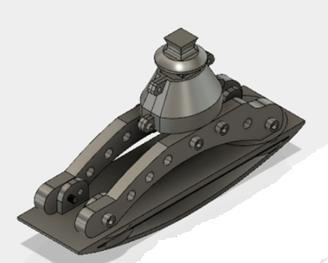
\includegraphics{protese}
\caption{Protótipo do pé protético desenvolvido pelo LBRSC.}
\label{Rotulo}
\end{figure}

Tanto quanto se sabe na Literatura, se conhece trabalho de robôs com pés curvos que possuem atuação limitada \cite{massachu}. Mas não se conhece humanoides completamente atuados que caminham com pés curvos permitindo o rolamento, semelhante ao ser humano. Esta será a grande contribuição do trabalho.

O embasamamento matemático dos métodos propostos será apresentado a seguir:


\subsection{Preview Control of ZMP}

O \emph{Preview Control of Zero-Moment Point} é um método seminalalítico de controle de caminhada bípede baseado em \emph{Model Predictive Control} (MPC) \cite{kajita2003}. Não apenas esse método foi implementado em vários robôs humanoides \cite{yi2016}, mas  também serve de base para técnicas no estado da arte \cite{tesemarcos,herdt2010}. Além disso, o LAB-SCA tem experiência no uso desse tipo de algoritmo de caminhada \cite{max22,tesemarcos}, de modo que o \emph{Preview Control of ZMP} será um ponto de partida para esse trabalho. Nessa subseção, apresentar-se-á uma introdução teórica a esse método.

A inspiração para o uso de MPC advém do fato de que, durante a caminhada, mudanças instantâneas ocorrem no polígono de suporte devido aos pés do robô fazerem e quebrarem contato com o chão. Com isso, é interessante que o controlador de caminhada anticipe a referência futura de ZMP ao mover o ZMP antes que uma mudança repentina de polígono de suporte aconteça.

Controle Preditivo Baseado em Modelo (MPC) é uma abordagem moderna de controle ótimo em que o comportamento futuro do sistema dinâmico é previsto através da integração de um modelo matemático. A seguir, deduz-se as equações apenas para o eixo de coordenadas \( x \), dado que estendê-las para o eixo \( y \) é trivial.

Primeiramente, considere controle direto sobre a sobre-aceleração (i.e. derivada da aceleração) do CM do robô  \( \dddot{x} \), então a evolução temporal do CM é ditada pela Cinemática. Assumindo-se a hipótese de segurador de ordem zero sobre um passo de tempo de duração \( T \), pode-se obter o seguinte modelo de tempo discreto para a dinâmica do CM:
\begin{equation}
\mathrm{\mathbf{x}}[k+1] = \begin{bmatrix}
1 & T & T^2/2 \\ 0 & 1 & T \\ 0 & 0 & 1
\end{bmatrix} \mathrm{\mathbf{x}}[k] + \begin{bmatrix}
T^3/6 \\ T^2/2 \\ T
\end{bmatrix} \dddot{x}[k],
\label{eq:discrete_dynamics_x}
\end{equation}
em que \( \mathrm{\mathbf{x}}[k] = \left[ x[k] \ \dot{x}[k] \ \ddot{x}[k] \right]^T \). Além disso, se a altura do CM \( h \) é mantida constante e a variação do momento angular é ignorada, a dinâmica do ZMP segue o conhecido modelo de pêndulo invertido \cite{kajita2001}:
\begin{equation}
z_x[k] = \begin{bmatrix}
1 & 0 & -h/g
\end{bmatrix} \mathrm{\mathbf{x}}[k],
\label{eq:zmp}
\end{equation}
em que \( g \) é a aceleração da gravidade. A predição do comportamento futuro do sistema em um horizonte de \( N \) passos de tempo, dada uma sequência de comandos \( \dddot{\mathrm{\mathbf{X}}}[k] = \left[\dddot{x}[k|k] \ \cdots \ \dddot{x}[k+N-1|k] \right]^T \), pode ser obtida por:
\begin{equation}
\mathrm{\mathbf{X}}[k] = \begin{bmatrix}
x[k+1|k] \\
%x[k+2|k] \\
\vdots \\
x[k+N|k]
\end{bmatrix} = \mathrm{\mathbf{P}}_{ps} \mathrm{\mathbf{x}}[k] + \mathrm{\mathbf{P}}_{pu} \dddot{\mathrm{\mathbf{X}}}[k], \
\dot{\mathrm{\mathbf{X}}}[k] = \begin{bmatrix}
\dot{x}[k+1|k] \\
%\dot{x}[k+2|k] \\
\vdots \\
\dot{x}[k+N|k]
\end{bmatrix} = \mathrm{\mathbf{P}}_{vs} \mathrm{\mathbf{x}}[k] + \mathrm{\mathbf{P}}_{vu} \dddot{\mathrm{\mathbf{X}}}[k],
\label{eq:dx_pred}
\end{equation}
\begin{equation}
\ddot{\mathrm{\mathbf{X}}}[k] = \begin{bmatrix}
\ddot{x}[k+1|k] \\
%\dot{x}[k+2|k] \\
\vdots \\
\ddot{x}[k+N|k]
\end{bmatrix} = \mathrm{\mathbf{P}}_{as} \mathrm{\mathbf{x}}[k] + \mathrm{\mathbf{P}}_{au} \dddot{\mathrm{\mathbf{X}}}[k], \
\mathrm{\mathbf{Z}}_x[k] = \begin{bmatrix}
z_x[k+1|k] \\
%z_x[k+2|k] \\
\vdots \\
z_x[k+N|k]
\end{bmatrix} = 
\mathrm{\mathbf{P}}_{zs} \mathrm{\mathbf{x}}[k] + \mathrm{\mathbf{P}}_{zu} \dddot{\mathrm{\mathbf{X}}}[k],
\label{eq:zx_pred}
\end{equation}
em que as matrizes \( \mathrm{\mathbf{P}}_{ps} \), \( \mathrm{\mathbf{P}}_{pu} \), \( \mathrm{\mathbf{P}}_{vs} \), \( \mathrm{\mathbf{P}}_{vu} \), \( \mathrm{\mathbf{P}}_{as} \), \( \mathrm{\mathbf{P}}_{au} \), \( \mathrm{\mathbf{P}}_{zs} \), e \( \mathrm{\mathbf{P}}_{zu} \) podem ser determinadas usando as equações \eqref{eq:discrete_dynamics_x} e \eqref{eq:zmp}. Assim, rastreia-se uma trajetória futura de ZMP de referência sobre um horizonte através do uso da seguinte função de custo:
\begin{equation}
J \left( \dddot{\mathrm{\mathbf{X}}}[k] \right) = \frac{\alpha}{2} || \dddot{\mathrm{\mathbf{X}}}[k] ||^2 + \frac{\gamma}{2} || \mathrm{\mathbf{Z}}_{r,x}[k] - \mathrm{\mathbf{Z}}_x[k] ||^2,
\label{eq:optimization_preview}
\end{equation}
em que os pesos \( \alpha \) e \( \gamma \) penalizam o uso de sobre-aceleração e o erro de rastreio de ZMP, respectivamente. Além disso, \( \mathrm{\mathbf{Z}}_{r,x}[k] \) é a trajetória de referência de ZMP no eixo \( x \), i.e. \( \mathrm{\mathbf{Z}}_{r,x}[k] = \left[z_{r,x}[k+1] \ \cdots \ z_{r,x}[k+N] \right]^T \).

Para o máximo de estabilidade, o artigo original sugere escolher uma referência de ZMP poligonal que mantém o ZMP no meio do pé de suporte durante suporte simples e move o ZMP entre os pés durante suporte duplo \cite{kajita2003}. A hipótese implícita aqui é que o rastreio de ZMP é bom o suficiente para manter o ZMP sempre dentro do polígono de suporte, como exigido pelo critério de estabilidade de ZMP \cite{vukobratovic2004}. Porém, outro tipo de referência é mais interessante caso deseje-se reduzir consumo energético, conforme já explorado por pesquisadores do LAB-SCA \cite{max22}.

O algoritmo é usado em conjunto com um planejador de passos que escolhe as posições dos pés de acordo com um objetivo de alto nível. A trajetória de sobre-aceleração é obtida através da solução do problema de otimização definido pela função de custo \eqref{eq:optimization_preview}, o qual possui solução analítica:
\begin{equation}
\dddot{\mathrm{\mathbf{X}}}[k] = \left( \mathrm{\mathbf{P}}^T_{zu} \mathrm{\mathbf{P}}_{zu} + \frac{\alpha}{\gamma} \mathrm{\mathbf{I}}_N \right)^{-1} \mathrm{\mathbf{P}}^T_{zu} \left( \mathrm{\mathbf{Z}}_{r,x} - \mathrm{\mathbf{P}}_{zs} \mathrm{\mathbf{x}}[k] \right),
\end{equation}
em que \( \mathrm{\mathbf{I}}_N \) representa a matriz identidade de tamanho \( N \). Como não é possível controlar diretamente sobre-aceleração em um robô com atuadores de posição, como o Robotis OP2, é necessário reconstruir a trajetória de CM usando \eqref{eq:dx_pred}. Para mais informações sobre como implementar essa técnica em um robô real, sugere-se ler \cite{tesemarcos}.

Um ponto que se deve destacar é que esse método se baseia no consagrado 3D-LIPM \cite{kajita2001}, que mantém a altura do CM constante para resultar numa dinâmica linear. Entretanto, alguns pesquisadores tem explorado prescrever uma trajetória para a altura do CM \cite{herdt2013}, de modo que o algoritmo de controle deve lidar com uma dinâmica linear variante no tempo:
\begin{equation}
z_x\left[ k \right] = x \left[ k \right] - \frac{h}{\ddot{z}_{r,CM}\left[ k \right] + g} \ddot{x} \left[ k \right]
\end{equation}
em que \( \ddot{z}_{r,CM}[k] \) é a trajetória prescrita para a altura do CM. Conforme descrito em \cite{herdt2013}, uma formulação de MPC sem restrições lida facilmente com esse tipo de dinâmica. Nesse trabalho, pretende-se explorar a melhoria da eficiência energética da caminhada obtida com a variação da altura do CM, juntamente com o rolamento do pé, que será abordado na próxima subseção. Ambas características estão presentes na caminhada humana.

\subsection{Análise de energia para o rolamento}

Para uma análise de energia que considera a nova forma geométrica dos pés robótico, propõe-se usar o método proposto em  \cite{adamczyk2013}. Na figura 3, é exemplificada o efeito de variação de raio $\rho$ e comprimento l de um pé em forma de  arco, em um modelo de caminhada simples. 

\begin{figure}[!htb]
\centering
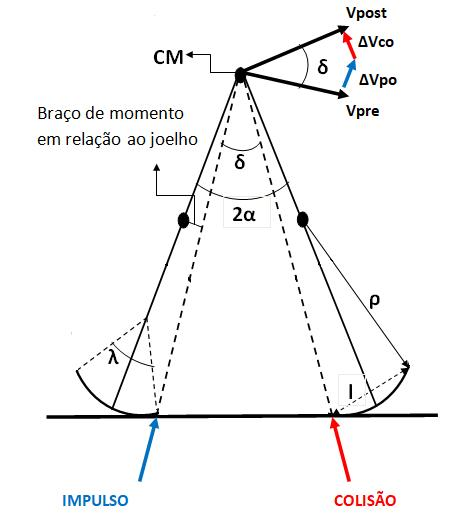
\includegraphics{centromassa}
\caption{ Modelo de caminhada.}
\label{Rotulo}
\end{figure}


Na figura 3 para a transição dos passos é considerado como trabalho positivo o impulso e trabalho negativo a colisão, para redirecionar a velocidade CM. O redirecionamento (representado pelo ângulo $\delta$) é determinado pela distância entre os pontos de contato do solo para os dois arcos.

Para um valor maior de redirecionamento do CM é necessário mais trabalho (mais energia). A mudança de velocidade devido ao impulso e a colisão são mostrados como  $\Delta v_{PO}$ e $\Delta v_{CO}$, respectivamente. 

Mantendo constante o comprimento do  passo, determina-se tanto o ângulo entre as pernas (2$\alpha$) quanto o ângulo mínimo  de redirecionamento ($\delta$). Os impulsos redirecionam o CM com uma  velocidade de pré transição ($ v_{pre}$) para a velocidade de meio transição ($v_{mid}$), já a colisão redireciona o CM com uma velocidade de pós transição ($v_{post}$). 

Sendo o comprimento do pé dado pela relação relação l=2$\rho$sin($\lambda$/2) , onde $\lambda$ é o ângulo do arco do pé. Para encontrar  $\delta$, usa-se a relação:

\begin{equation}
\tan\frac{\delta }{2}=\frac{\rho\sin (\alpha-\frac{\lambda}{2})+(1-\rho)sin\alpha}{\rho\cos (\alpha-\frac{\lambda}{2})+(1-\rho)\cos\alpha }\approx\alpha-\frac{l}{2}
\end{equation}

Para a marcha se manter estável a magnitude do trabalho da colisão deve ser igual a do trabalho do impulso, encontrado por:

\begin{equation}
W=\frac{1}{2}M(v_{mid})^2-\frac{1}{2}M(v_{post})^2=\frac{1}{2}M(v_{post})^2\tan^2\frac{\delta}{2}
\end{equation}

%Portanto, o módulo do trabalho tanto na colisão quanto no impulso é:

\begin{equation}
W\approx\frac{1}{2}M(v_{post})^2(\alpha-\frac{l}{2})^2
\end{equation}





\newpage

\section{Objetivos}

Conforme apresentado anteriormente, no estágio atual da pesquisa de robôs humanoides, alguns fatores e parâmetros são fundamentais para permitir o desenvolvimento de novos modelos de marcha. Dentre eles podem ser considerados materiais com alto amortecimento, uma geometria que permita rolamento e consequentemente diminuição da força de impacto e diminuição de gastos energéticos.

Este  trabalho efetivamente juntará conhecimentos de duas áreas, Biomecânica e Robótica através de uma colaboração de dois laboratórios. Portanto no presente trabalho pretende-se adequar o pé protético desenvolvido pelo LBRSC e adaptá-lo em um robô existente no LAB-SCA, com o objetivo de sua marcha ficar energeticamente mais eficiente. 

Para isso, segue os  seguintes objetivos específicos:
\begin{enumerate}
\item 	Identificar, a partir da técnica de Cinemetria e Dinamometria por sensores de pressão nos pés, os parâmetros do robô Robotis OP2.

\item	Desenvolver pés robóticos que permitam diminuição do gasto energético e absorção do impacto.

\item	Implementação dos pés  na caminhada do robô (Robotis OP2).
 \end{enumerate}
Finalmente, como objetivo institucional busca-se o fortalecimento da colaboração entre os dois laboratórios(LBRSC e LAB-SCA). Espera-se que este trabalho também fomente trabalhos, pelo menos um de conclusão de curso e de iniciação científica, em algum dos temas: Cinemetria, identificação de parâmetros e instrumentação do pé. 

Também espera-se a publicação dos temas: identificação de robô humanoide, projeto mecânico do pé com rolamento, caminhada do robô humanoide com rolamento e instrumentação do pé. 

Pretende-se a publicação nas seguintes conferências:
\begin{itemize}
   \item International Congress of Mechanical Engineering (COBEM);
   \item Congresso Nacional de Engenharia Mecânica (CONEM);

\item International Symposium on Dynamic Problems of Mechanics (DINAME);

\item Ibero Latin American Congress on Computational Methods in Engineering (CILAMCE);

\item Latin Americam Robotics Symposium (LARS);

\item IEEE RAS Internacional Conference on Humanoids Robots(HUMANOIDS);

\item International Conference on Robotics and Automation (ICRA);

\item International Conference on Intelligent Robots and Systems(IROS).
 \end{itemize}

Pretende-se publicação nos seguintes periódicos:
\begin{itemize}
\item Journal Of Mechanisms and Robotics (Qualis B1 engenharias III);

\item Journal of Intelligent \& Robotics Systems (Qualis B1 engenharias III);

\item IEEE/ASME Transactions on Mechatronics (Qualis A1 engenharias III).
 \end{itemize}
%\newpage

\section{Plano de trabalho}

A.	Revisão bibliográfica;

B.	Utilizar a técnica de cinemetria nos robôs do LAB-SCA para refinamento de parâmetros;

C.	Elaboração de algoritmo que permite rolamento do pé;

D.	Verificação em simulação da proposta de algoritmo de caminhada;

E.	Projeto mecânico do pé e fabricação;

F.	Implementação do algoritmo no robô;

G.	Cinemetria com o novo pé;

H.	Redação /defesa do exame de qualificação;

I.	Instrumentação;

J.	Testes e análises de resultados;

K.	Redação/defesa da tese.


\begin{table}[h!]
	\centering
	\caption{Cronograma de atividades detalhado.}
	\label{tab:Cronograma}
		\begin{tabular}{|c|C|C|C|C|C|C|C|C|C|C|C|}
		\hline
		\multirow{2}{*}{Semestre} &  \multicolumn{11}{c|}{Atividade} \\
		 & \multicolumn{1}{c}{A} & \multicolumn{1}{c}{B} & \multicolumn{1}{c}{C} & \multicolumn{1}{c}{D} & \multicolumn{1}{c}{E} & \multicolumn{1}{c}{F} & \multicolumn{1}{c}{G} & \multicolumn{1}{c}{H} & \multicolumn{1}{c}{I} & \multicolumn{1}{c}{J} & K 	\\
		  \cline{2-12}
			1 & \cellcolor{gray!50} & \cellcolor{gray!50} &  &  &  &	 &  &  &  &  & \\
			\cline{2-12}
			2 &  & \cellcolor{gray!50} & \cellcolor{gray!50} & \cellcolor{gray!50} &  &	&  &  &  &  & \\
			\cline{2-12}
			3 &  &  &  &  & \cellcolor{gray!50} & 	&  &  &  &  & \\
			\cline{2-12}
			4 &  &  &  & &  &	\cellcolor{gray!50} & \cellcolor{gray!50} & \cellcolor{gray!50} &  &  & \\
			\cline{2-12}
			5 &  &  &  &  &  &	&  &  & \cellcolor{gray!50} &  & \cellcolor{gray!50}\\
			\cline{2-12}
			6 &  &  &  &  &  &	&  &  &  & \cellcolor{gray!50} & \cellcolor{gray!50} \\
					
			\hline
	\end{tabular}
\end{table}

%\newpage

\section{Material e métodos}

Para a excução do projeto proposto são necessários os seguintes recursos materiais:

1.	O robô humanoide (Robotis OP2) comprado pelo  projeto FAPESP 2016/03647-3, utilizado na tese de doutorado \cite{tesemarcos};

2.	Acesso ao LAB-SCA (Laboratório de Sistemas de Controle autônomos), o qual contribuirá com equipamentos de confecção.

3.	 Acesso ao LBRSC (Laboratório de Biomecânica, Robótica e Simulação Computacional), o qual contribuirá com a Cinemetria.

4.	Licença do software Matlab, obitodo pelo projeto FAPESP 2016/03647-3.

5.	Modelo de simulação do Darwin desenvolvido na tese de doutorado dentro do contexto do projeto FAPESP 2016/03647-3.

6.	Biblioteca com acesso eletrônico aos periódicos de interesse nas áreas da proposta.



A metodologia seguida neste trabalho consiste em uma primeira etapa de experimentos para identificação de parâmetros de um robô Robotis OP2, para o qual existe um modelo de caminhada em um simulador.

Após isso propõe-se um novo modelo de caminhada que considerará o rolamento, com a construção de um novo pé. Posteriormente, serão feitas simulações dinâmicas tanto para validação do dispositivo construído quanto para a caminhada. Por fim, a implementação desse dispositivo no humanoide Robotis OP2.



%\newpage

\section{Forma de análise dos resultados}

Pretende-se aproveitar a experiência da instituição em identificação \cite{gripp}, a partir disso os dados obtidos por Cinemetria e Dinamometria serão analisados por algum método de identificação na abordagem amostrada por \cite{ident2014,ident2017}.

No projeto mecânico do pé robótico será verificado a resistência mecânica de cada componente considerando um carregamento estático. Para as forças dinâmicas será realizada uma análise modal, utilizando o método de elementos finitos.

A caminhada com o novo pé será analisada por um simulador, por experiência do LAB-SCA pretende utilizar o simulador Gazebo que atualmente é usado para o modelo de simulação do Robotis OP2.

O uso de simulação será usado numa etapa preliminar de resultados, além disso possui vantagens por fornecer diversos dados que são dificilmente extraídos de um experimento real. Como as forças e torques de todos os componentes do robô. 

Essas informações são essênciais para uma  avaliação precisa do consumo energético, de modo a validar o aumento da eficiência energética da caminhada proposta.

Posteriormente, o experimento da cinemetria será repetido para a caminhada que utiliza os pés curvos, para uma validação experimental do algoritmo e do dispositivo desenvolvidos neste trabalho.

Inicialmente a instrumentação do pé será validada em bancada, posteriormente o pé sensoriado será integrado no robô e será realizados novos experimentos com esse pé. 


\newpage

%\section{Referências}


\printbibliography
\end{document}